\chapter{Informationsbeschaffung}
\label{Informationsbeschaffung}
 In einer ersten Phase wurde ein Zeitraum zur Informationsbeschaffung festgelegt. Dieser Abschnitt ist einerseits für die Themeneinarbeitung und anderseits für die Abgrenzung der Aufgabe und der Ziele erforderlich.

Nachfolgend werden die wichtigsten Erkenntnisse der Informationsbeschaffung erläutert, die massgebend für die Konzeption in Kapitel \ref{chap:Konzeption} und die Realisierung in Kapitel \ref{chap:Realisierung} sind. Dabei werden zu einzelnen Komponenten und Verfahren Stellung genommen und eruiert, ob diese sich für das Projekt eignen. Des Weiteren wird relevante Software erläutert, die für die Realisierung nötig ist. Ein weiterer Abschnitt behandelt bereits bestehende Lösungen, die den aktuellen Stand der Technik aufzeigen. Die einzelnen Unterkapitel wurden nach Funktionsblöcken unterteilt.

\section{Entfernungsmessung}
\label{sec:Entfernungsmessung}
In diesem Unterkapitel wird der bestehende 3D-Laserscanner Velodyne VLP-16 analysiert. Dabei werden wichtige Spezifikationen erläutert. Anhand der Spezifikationen und Schnittstellen des Velodyne werden in den nächsten Unterkapitel weitere Komponenten eruiert.   

\subsection{Velodyne VLP-16 Puck}
\label{subsec:Velodyne}
Beim Velodyne VLP-16 Puck handelt es sich um einen Echtzeit 3D-Laserscanner, der auf dem \ac{LIDAR}-Verfahren basiert. Nachfolgende Angaben entstammen aus dem Datenblatt, wenn nicht anders referenziert. \protect\cite{velodyne}

Der VLP-16 bietet insgesamt 16 Laser-/Detektorpaare, die in Abbildung \ref{fig:angleVLP} ersichtlich sind. Mit diesen wird in horizontaler Lage ein Messbereich von 360$^\circ$  erreicht. Dies wird dadurch ermöglicht, dass der Laserscanner sich intern mit 5 - 20 Rotationen pro Sekunde (300 - 1200 RPM) um die eigene Achse dreht. Die Rotationsgeschwindigkeit ist softwaremässig einstellbar. Dabei wird mit einer horizontalen Auflösung von 0.1$^\circ$ – 0.4$^\circ$ gerechnet. Diese Auflösung begründet sich auf die nötige Zeit eines Messdurchgangs. Um alle 16 Laser abzufeuern und wieder zu entladen dauert es 56 $\mu$s.
Da die 16 Laser mit je 2$^\circ$ Unterschied ausgerichtet sind ergibt sich daraus ein vertikaler Messbereich von 30$^\circ$ mit einer vertikalen Auflösung von 2$^\circ$. 

Ein wichtiger Punkt ist somit, dass im stationären Zustand zwischen den Laserstrahlen keine Messpunkte ermittelt werden können. Um dies zu ermöglichen, muss der Laserscanner seine Position verändern.

\begin{figure}[H]
	\centering
	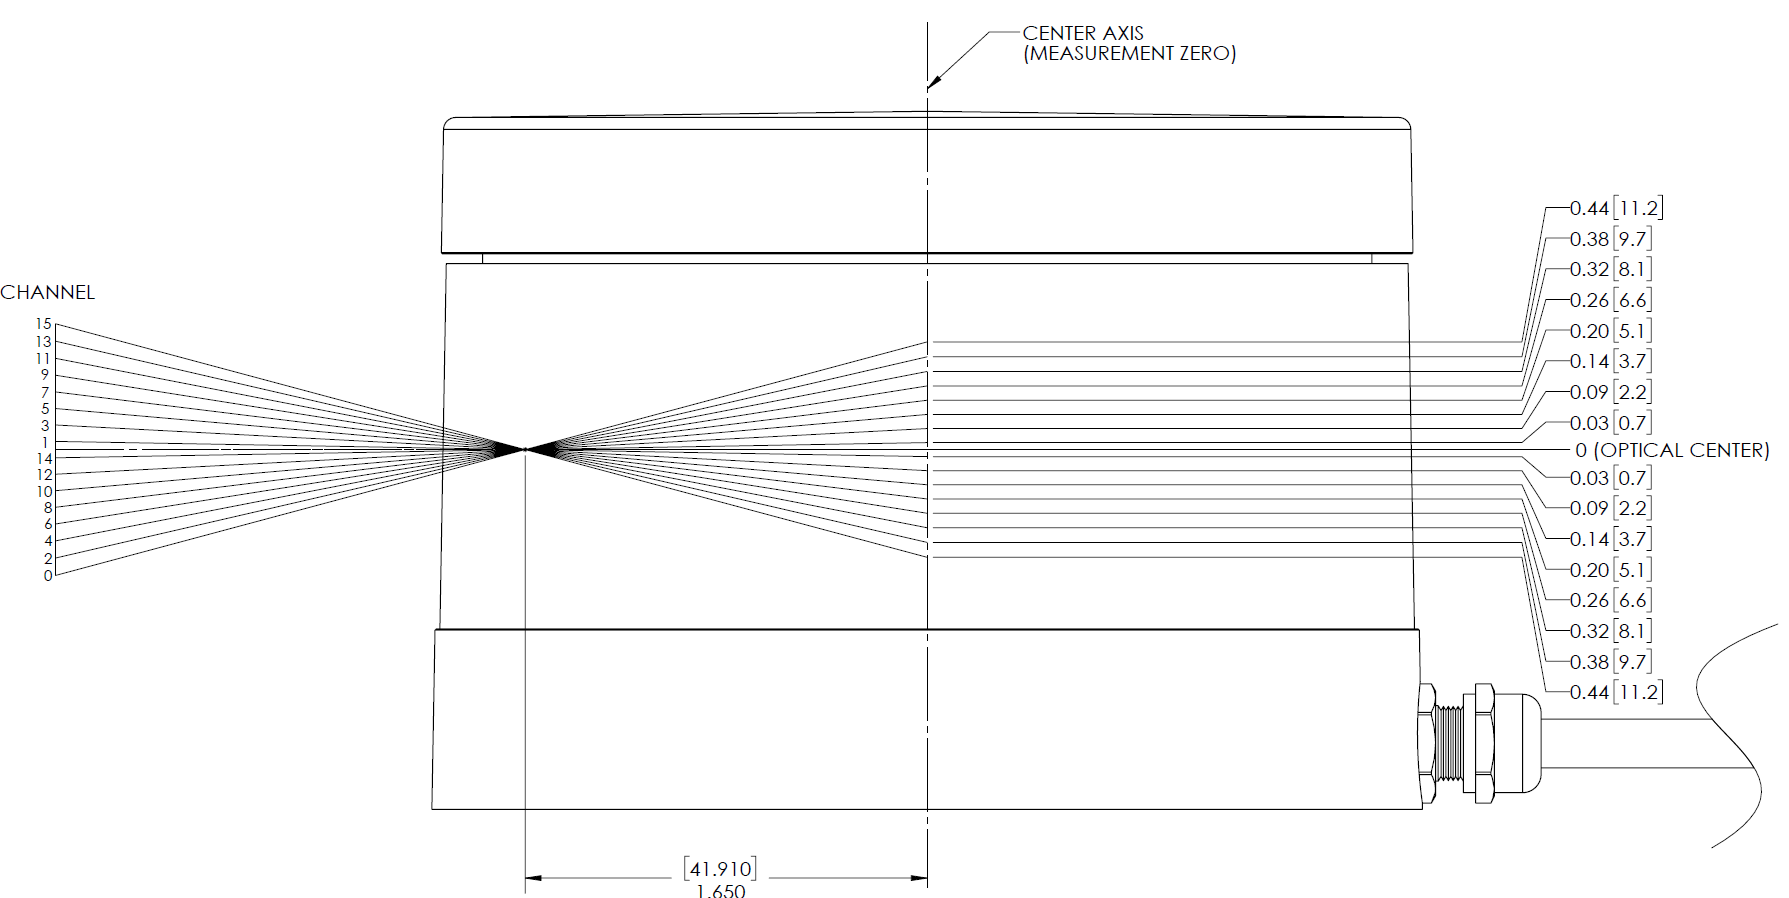
\includegraphics[width=0.8\textwidth]
	{resources/velodyne_channels.PNG}
	\caption[Laserstrahlen des Velodyne  VLP-16]{Laserstrahlen des Velodyne  VLP-16} \protect\cite{velodyne}
	\label{fig:angleVLP}
\end{figure}

Eine relevante Eigenschaft dieses Laserscanners ist die grosse Messdistanz, die Distanzen zwischen 0.3 m bis 100 m ermöglichen. Dabei ist die typische Toleranz +/- 3 cm. Der Reflektionsgrad wird in 256-bit Auflösung angegeben, d.h. dass der Sensor aus der zurückgesendeten Laserimpulsen die Intensität messen kann.

Der VLP-16 benötigt eine separate Interface Box, mit der die Speisung und die Datenschnittstellen zu einem 8-adrigen Kabel zusammengeführt werden. Die Adern 1-4 werden für die Ethernet Datenübertragung benötigt. Die Adern 5 und 6 sind nur bei zugeschaltetem \ac{GPS} nötig, ansonsten sind diese unbenutzt. Die stabilisierte 12 Volt Spannung wird über die Adern 7 und 8 zugeführt. Die Interface Box ist in Abbildung \ref{fig:InterfaceBox} ersichtlich. Diese besitzt folgende Anschlüsse; eine 12 Volt Speisung, einen Ethernet RJ45-Anschluss und eine \ac{GPS} Schnittstelle. Für die typische Leistungsaufnahme des Sensors wird 8 Watt angegeben. Aus einem Messaufbau konnte bei 12 Volt Speisespannung einen Strom von 0.6 Ampere ermittelt werden. Im Einschaltmoment kann der Strom kurzzeitig auf 0.9 Ampere ansteigen. Dies muss bei der Dimensionierung der Speisung beachtet werden.  

\begin{figure}[H]
	\centering
	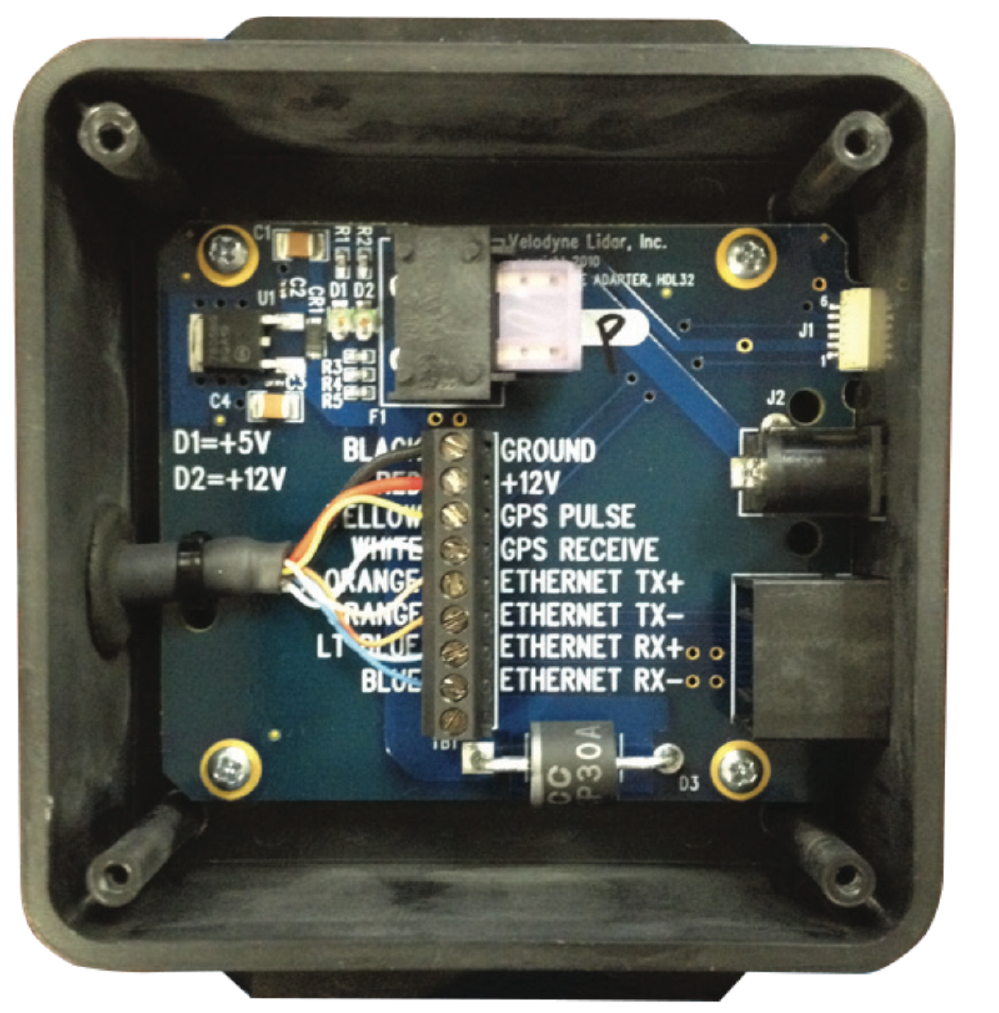
\includegraphics[width=0.5\textwidth]
	{resources/InterfaceBox.PNG}
	\caption[Ansicht auf die Interfacebox]{Ansicht auf die Interface Box} \protect\cite{velodyne}
	\label{fig:InterfaceBox}
\end{figure}

Über die Ethernetverbindung werden die Daten- und Positionspakete vom Velodyne an den Computer übermittelt. Dabei werden für die zwei verschiedenen \ac{UDP} Pakete die Ports 2368 und 8308 gebraucht. Nachfolgend wird in Abbildung \ref{fig:datapakets} der Aufbau eines Datenpakets dargestellt.

\begin{figure}[H]
	\centering
	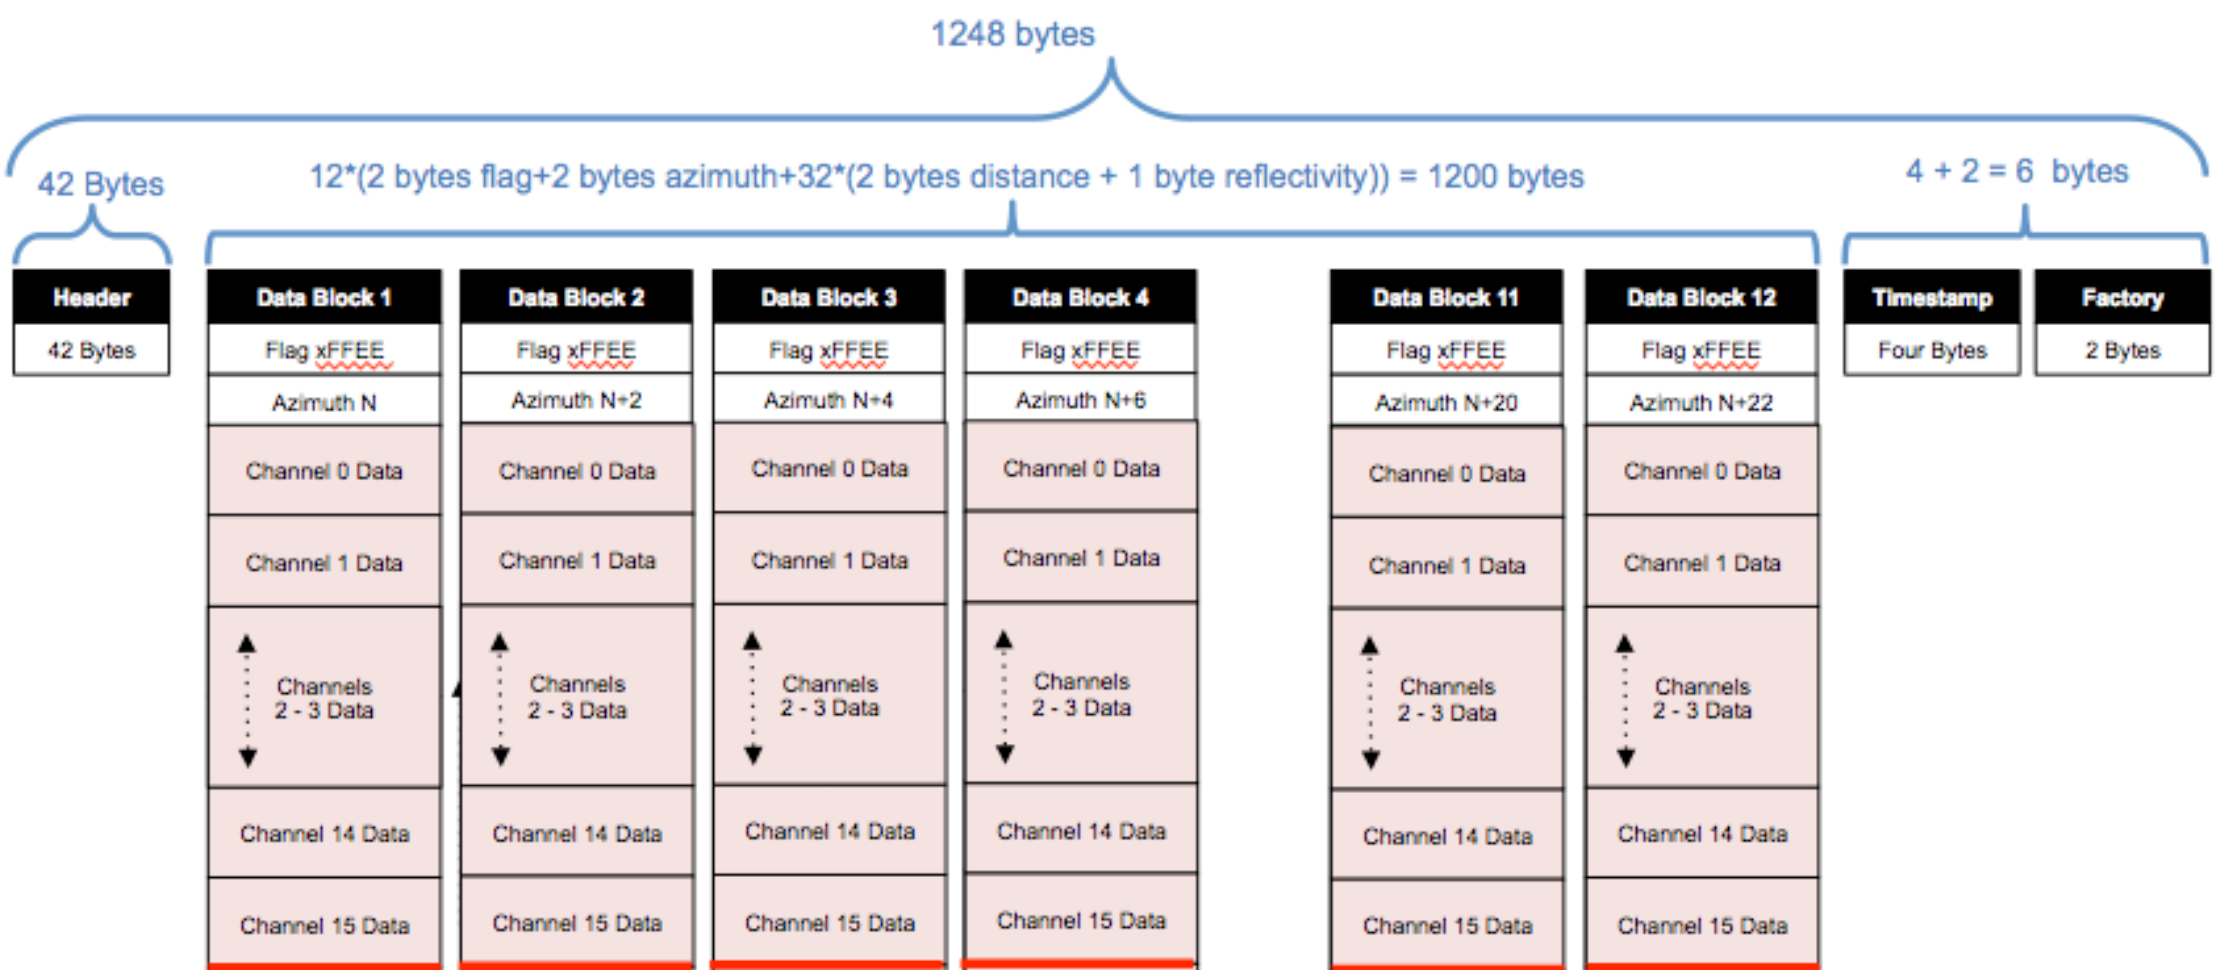
\includegraphics[width=1.0\textwidth]
	{resources/datapakets.PNG}
	\caption[Aufbau Datenpaket]{Aufbau Datenpaket} \protect\cite{velodyne}
	\label{fig:datapakets}
\end{figure}

 Jedes Paket besitzt einen 42-Byte Header und einen Datenblock, der aus Laserrückgabewert, kalibrierten Reflektionsgrad, Azimutwert und Zeitstempel besteht. Ein einzelnes Datenpaket besitzt die Grösse von 1248 Bytes und beinhaltet die Datensätze aller 16 Laserkanäle. Die typische Datenübertragungsrate wird angegeben mit 8 Mbit/s angegeben.

\section{Stand der Technik}
 \label{sec:Vorzeigeprojekte}
 Dieses Kapitel dient als Vorstudie über den Einsatz des Velodyne VLP-16 durch bereits bestehende Projekte. Dabei werden zwei verschiedene Konfigurationen betrachtet und dazu entsprechend Vor- und Nachteile erläutert. Es handelt sich hierbei um zwei Teams, welche an der \ac{EnRicH} 2017 teilgenommen haben und als State-of-the-Art Projekte betrachtet werden.
 
 \subsection{IMM MSAS Team MSS Warschau}
 \label{subsec:IMM}
Das Institute of Mathematical Machines (IMM) in Warschau hat den Velodyne VLP-16 an einer endlos drehenden Konstruktion befestigt. Dabei ist der Sensor nicht in der üblichen Lage (Ausrichtung XY-Ebene), sondern um 90$^\circ$ abgedreht (Ausrichtung YZ Ebene). In Abbildung \ref{fig:imm} ist die entsprechende Konfiguration abgebildet. 

   \begin{figure}[H]
	\centering
	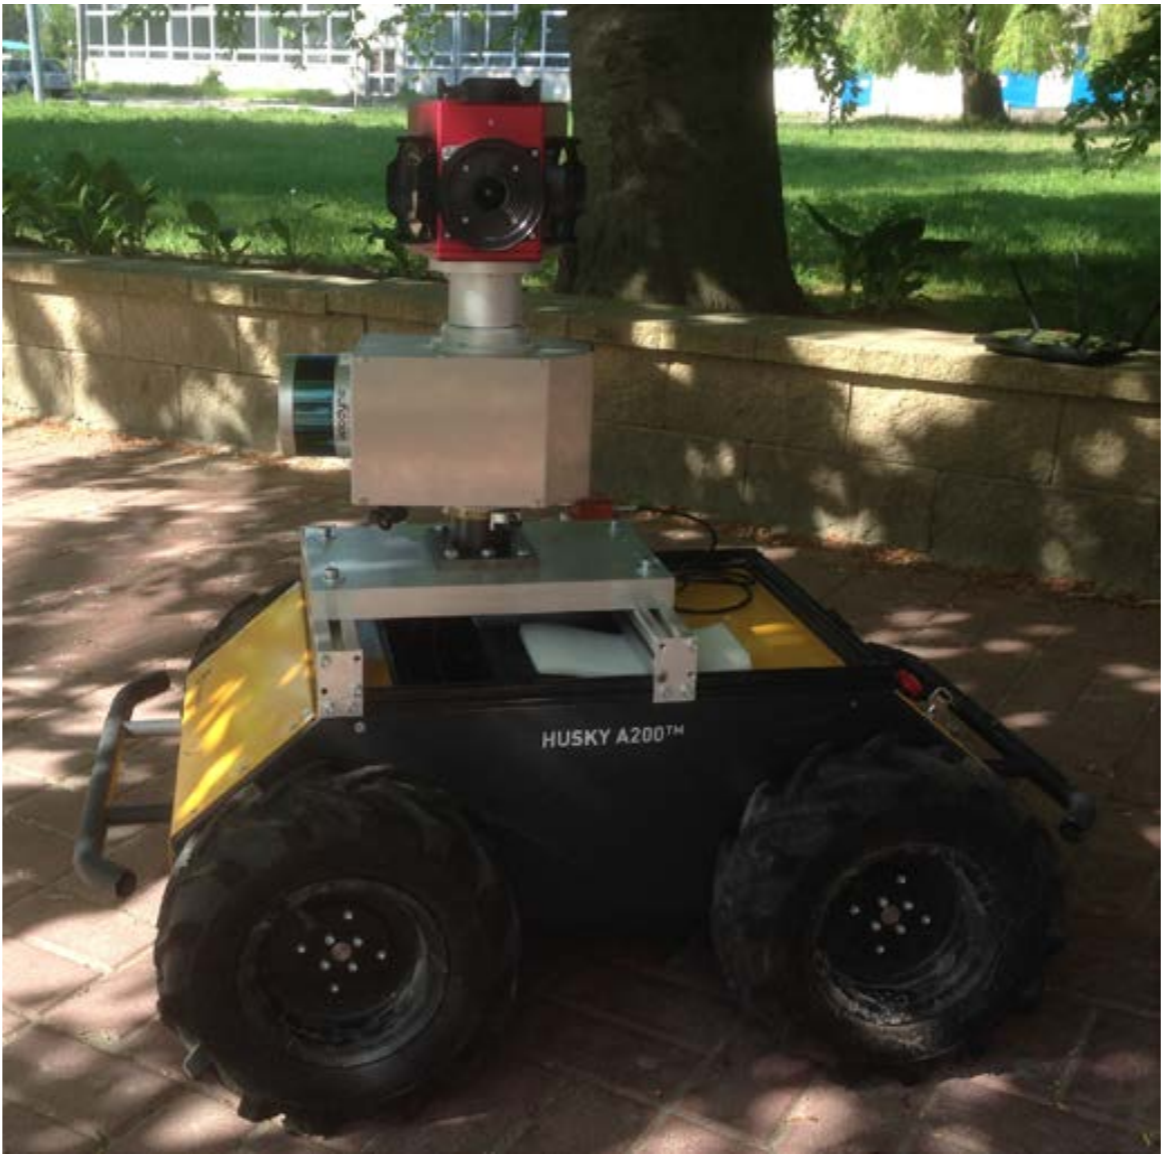
\includegraphics[width=0.6\textwidth]
	{resources/IMM.PNG}
	\caption[Roboter des Team IMM EnRicH]{Roboter des Team IMM an der EnRicH} \protect\cite{IMM}
	\label{fig:imm}
\end{figure}

In der nachfolgenden Betrachtung wird vom Koordinatensystem der Abbildung \ref{fig:imm} ausgegangen.
Das Team nutzt bei dieser Konfiguration die begrenzte Auflösung des Sensors besser aus. Die vertikale und horizontale Auflösung wechseln dabei. Ist die Konstruktion nicht drehend, kann er in der Vertikalen den Bereich 360$^\circ$ mit der Auflösung von 0.01$^\circ$ - 0.04$^\circ$ messen. In der Horizontalen kann der Bereich 30$^\circ$ mit 2$^\circ$ aufgelöst werden. 

Der Vorteil dieser Konfiguration wird jedoch erst durch die Rotation um die Z-Achse deutlich. Wird der Sensor nun kontinuierlich um die Z-Achse gedreht, verschieben sich die 16 horizontalen Laserstrahlen mit der Umdrehungsgeschwindigkeit der Konstruktion. Einerseits bewegt sich der 30$^\circ$ grosse Messkegel durch den Raum und kann somit 360$^\circ$ in der Horizontalen vermessen. Anderseits kann durch die interne Rotation des Sensors 360$^\circ$  in der Vertikalen ausgemessen werden. Die schlechtere Auflösung von 2$^\circ$ kann somit kompensiert werden, da sich die Lasterstrahlen kontinuerlich verschieben. Diese Konfiguration ermöglicht eine detaillierte Messung, da jeder Punkt im Raum von 16 Laserstrahlen mit der Auflösung zwischen 0.1$^\circ$ - 0.4$^\circ$ durchlaufen wird. 

Die oben erläuterte Betrachtung gilt jedoch nur, wenn die Umdrehungsgeschwindigkeit der Konstruktion bedeutend langsamer als die interne Umdrehungsgeschwindigkeit des Sensor ist. Ansonsten besteht die Gefahr, dass die Reflektion des Laserstrahls nicht detektiert werden kann. Die Auflösung ist direkt von der Umdrehungsgeschwindigkeit der Konstruktion abhängig. Es wird zusätzlich davon ausgegangen, dass keine zusätzliche Translation, d.h. Bewegung des Roboters, stattfindet. Diese Konfiguration eignet sich somit, wenn das zu vermessende Gelände bekannt ist. Dadurch können vordefinierte Positionen angesteuert werden, an denen eine halbe Umdrehung ausreicht, um eine räumliche Messung an der definierten Position zu erstellen. 

Weiter wird in der obigen Betrachtung die Abweichung zur Drehachse komplett vernachlässigt. Es entsteht ein Messfehler, der dem Abstand des Sensors zur Drehachse entspricht. Ein weiterer Messfehler kann durch Translation entstehen, wenn sich das Fahrzeug bewegt. Diese zwei Messfehler lassen sich jedoch durch Koordinatentransformationen in ein festes Koordinatensystem verschieben. Die Schwierigkeit dabei ist, die exakten Messewerte mittels einem Drehencoder und einer \ac{IMU} zum jeweiligen Zeitpunkt zu ermitteln. 

Ein Nachteil für die Aufgabenstellung ist, dass bei dieser Konfiguration im freien Feld viele Messpunkte ins Leere messen, da himmelwärts (Richtung Z-Achse) keine Reflektion entsteht. Auch Messpunkte in Richtung negative Z-Achse müssen gefiltert werden, da ansonsten ständig die Oberfläche des Roboter selbst reflektiert wird.

\subsection{Hector Tracker Team Hector Darmstadt}
 \label{subsec:hector}
Das Team Hector der Universität Darmstadt besitzt auf dem Hector Tracker eine weitere Konfigurationsmöglichkeit. Auch dieses Team arbeitet mit einem endlos drehenden Konstruktion. Bei nachfolgenden Betrachtungen wird vom Koordinatensystem in Abbildung \ref{fig:hector} ausgegangen. Der Velodyne VLP-16 befindet sich 45$^\circ$ abgeneigt zur XZ-Ebene. Dabei ist die Lage des Sensors zentral auf der Drehachse Z.

\begin{figure}[H]
	\centering
	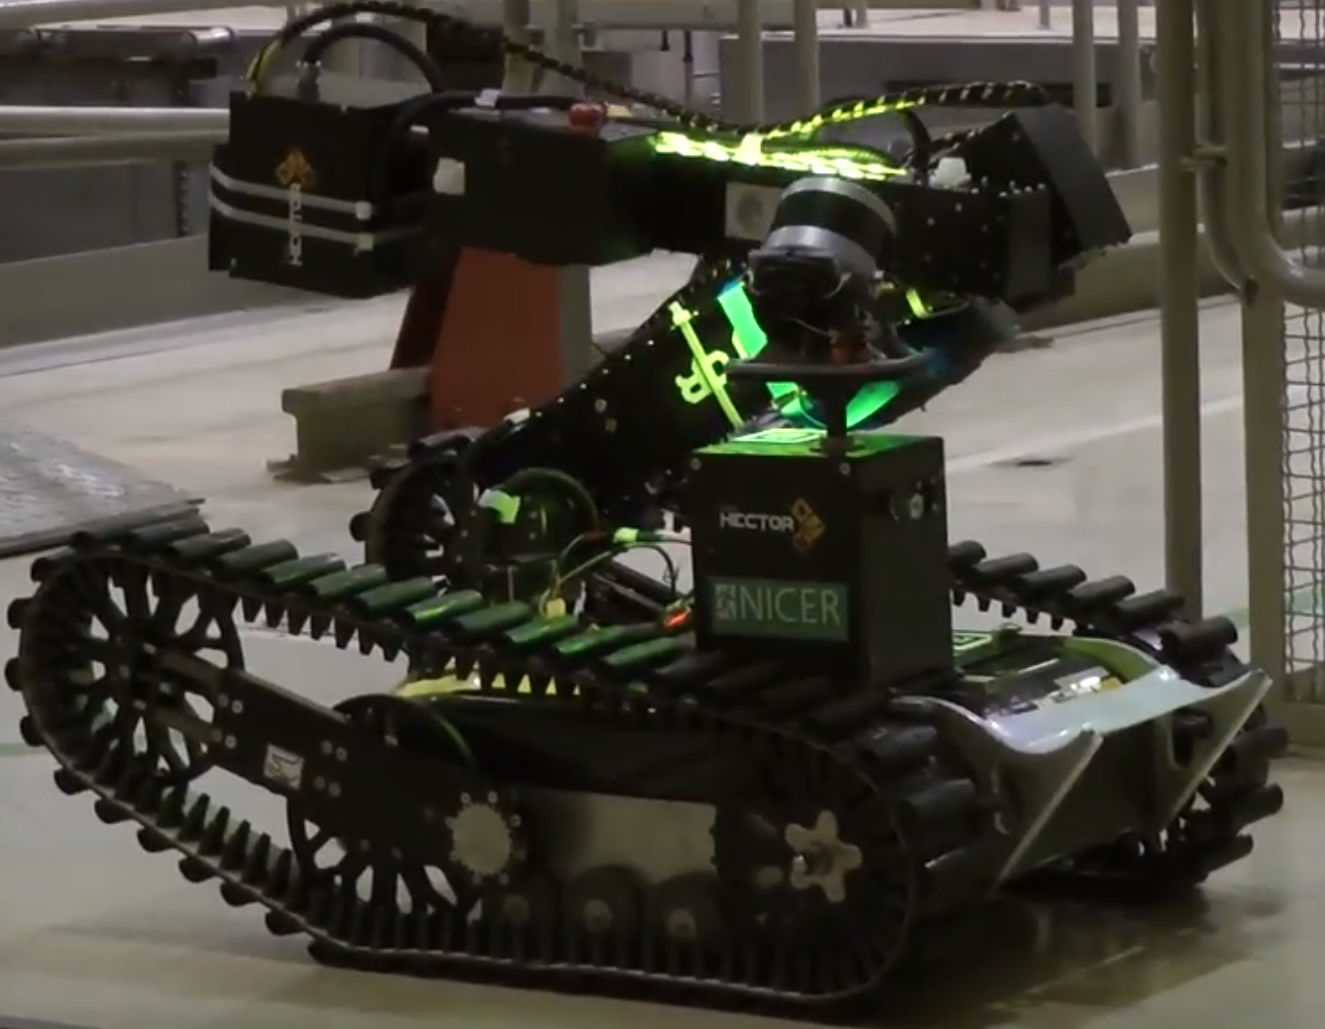
\includegraphics[width=0.7\textwidth]
	{resources/hector.PNG}
	\caption[Roboter des Team Hector EnRicH]{Roboter des Team Hector an der EnRicH} \protect\cite{hector}
	\label{fig:hector}
\end{figure}

Im stationären Zustand kann durch diese Konfiguration keine Verbesserung der Auflösung erreicht werden. Die Auflösungen bleiben erhalten, sind jedoch nun entsprechend der Neigung um 45$^\circ$ verschoben. Durch die Neigung des Sensors wird der Raum nicht gleichmäßig vermessen. Die räumliche Vermessung wird auch hier erst mit der Rotation um die Z-Achse ermöglicht. Gegenüber einer festen nicht drehenden Lösung besitzt diese Konfiguration somit den Vorteil, dass Messpunkte, welche sich zwischen den Laserstrahlen befinden, durch Drehen erreichen lassen. Dabei wird der 30$^\circ$ Messkegel durch die Rotation ständig im vertikalen Bereich hin- und hergeschoben.

Es kann während einer Umdrehung somit durch die Neigung von 45$^\circ$ und dem 30$^\circ$ Kegel des Sensors eine Abdeckung in der Vertikalen von 240$^\circ$ erreicht werden. Die horizontale Abdeckung bleibt hierbei weiterhin 360$^\circ$, da der Sensor die interne Rotation vollführt.

Auch bei dieser Betrachtung  muss die Umdrehungsgeschwindigkeit der Konstruktion bedeutend langsamer als die interne Umdrehungsgeschwindigkeit des Sensor sein. Die Auflösung bei dieser Konstruktion ist direkt zur Umdrehungsgeschwindigkeit abhängig. Des Weiteren muss bei dieser Konfiguration die Translation, d.h. die Bewegung des Roboters, noch separat korrigiert werden.  

Im Vergleich zum Projekt der IMM entstehen bei dieser Konfiguration weniger Messpunkte in Richtung des Roboters und in Richtung der Z-Achse (himmelwärts). Dies ist für Raum interne Messungen unvorteilhaft. Für die Messung im freien Feld ist diese Konfiguration besser geeignet, sofern sich keine hohe Objekte in der Nähe des Sensor befinden. 
 	
\subsection{Schlussfolgerung}
An der \ac{EnRicH} 2017 nutzen mehrere Teams den Velodyne VLP-16 mit unterschiedlichen Konfigurationen. Die zwei betrachteten Konfigurationen nutzen die Möglichkeit einer endlos drehenden mechanischen Konstruktion. Im Unterkapitel \ref{sec:Antriebsmoeglichkeiten} werden mögliche Antriebsmöglichkeiten für eine solche Konstruktion evaluiert. Eine endlos drehende Konstruktion benötigt ein spezielles Handling der Kabelführung, daher wird im Unterkapitel \ref{subsec:Schleifring} die Möglichkeit eines Schleifrings beschrieben. Beide Konfiguration besitzen Vor- und Nachteile bei der Umgebungserkennung. Um eine möglichst detaillierte Umgebungswolke zu erstellen müssen vorwiegend Translation und Rotation um die Drehachse kompensiert werden. Diese lassen sich durch Koordinatentransformation und entsprechender Sensorik ermöglichen. In Unterkapitel \ref{sec:position} werden dazu mögliche Varianten zur Positionsbestimmung erläutert.
  
\section{Software}
\label{sec:Software}
In diesem Kapitel wird die notwendige Software beschrieben. Es erläutert einerseits das \ac{ROS} und dessen Funktion im Projekt. Daneben werden weitere Softwareapplikationen und -packages erwähnt, welche für die Aufgabenstellung nützlich sind.

\subsection{ROS Robot Operating System}
\label{subsec:ROS}
Die gesamte Kommunikation mit Sensoren und Aktoren findet auf dem Packbot mit \ac{ROS} statt. Da das 3D-Laser-Modul auf dem Packpot, sowie selbstständig funktionieren soll, ist ROS nicht zwingend einsetzbar. Dennoch wurde für die Aufgabenstellung ROS gewählt. Im Zusammenhang mit Velodyne und 3D Mapping bietet ROS neben Visualisierungtools und bereits bestehender Treiber-Packages auch die Integrationen der \ac{PCL}. Die \ac{PCL} ist eine umfangreiche Softwarebibliothek, welche viele Funktionen und Codebeispiele bereit stellt, um Punktwolken zu erstellen.

Grundsätzlich wird \ac{ROS}, wegen seiner Nähe zu Linux Distributionen, auf einem Ubuntu Betriebssystem aufgesetzt und ist ein Software-Framework, dass die Programmiersprachen C++ und Python nutzt. Diese in 2007 entwickelte Open Source Software erhielt in den letzten Jahren ständig neue und überarbeitete Versionen.

Die Empfehlung von ROS und diversen Literaturen liegt bei der neusten Distribution ROS "Kinetic Kame". \cite{ROSprojects} Es handelt sich um eine Langzeitversion, welche bis 2021 Unterstützung bietet. Im Zug der ersten Versuchen mit ROS wurde auf einem Laptop mit \ac{AMD64}-Architektur gearbeitet. Auf diesem wurde ROS Kinetic Kame vollumfänglich ermöglicht. Damit das 3D-Lasermodul selbständig agieren kann, wird jedoch ein einbaubarer Einplatinencomputer benötigt. In in Unterkapitel \ref{sec:Datenverarbeitung} werden aktuelle Einplatinencomputer beschrieben . 

Während der Einarbeitung mit Kinetik Kame konnten einige Nachteile der Distribution festgestellt werden. Es wurde festgestellt, dass diverse Packages nur für \ac{AMD64}-Architekturen zur Verfügung stehen und nicht für \ac{ARM}-Architekturen. \cite{armhf_issues} Dies könnte zu Eingrenzungen während der Realisierung führen, daher werden nötige Packages geprüft.

\subsection{Velodyne Package}
Wie bereits im vorherigen Kapitel erwähnt, besitzt ROS ein Treiber-Package für den Velodyne VLP-16. Dieses Paackage wird für ARM- und AMD64-Architekturen ermöglicht. In der Abbildung \ref{fig:rosgraph} ist der Aufbau dieses Treibers mit dem ROS-Tool rqt-graph visualisiert. 

\begin{figure}[H]
	\centering
	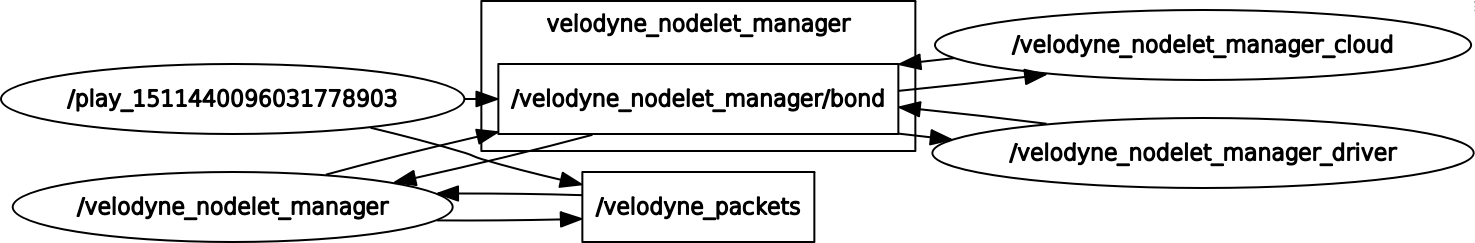
\includegraphics[width=1\textwidth]{resources/rosgraph.png}
	\caption[Velodyne Treiber aus rqt-graph ]{Velodyne Treiber aus rqt-graph}
	\label{fig:rosgraph}
\end{figure} 

Dieses Package vereinfacht die Sensordatenverarbeitung bedeutend. Mittels dem Package werden die hexadezimalen Rohdaten von den Ethernet-Datenpaketen aus Abbildung \ref{fig:datapakets} bereits ausgewertet und kalibriert zur Verfügung gestellt. Dabei laufen mehrere Programmsegmente (\textit{Nodes}) parallel. 

Für die Aufgabenstellung ist nur der Node velodyne\_packets relevant, da dieser den verarbeiteten Sensor-Datenstream zur Verfügung stellt. Es werden dabei zwei unterschiedliche Typen von \textit{Messages} kontinuerlich ausgegeben \textit{(published)}. Die Message \textit{velodyne\_packets (vom Typ: velodyne\_ msgs/VelodyneScan)} beinhaltet die Rohdaten eines einzelnen Laserstrahls. Die Message \textit{velodyne\_points (vom Typ: sensor\_msgs/PointCloud2)} beinhaltet die angesammelten Datenpunkte, welche bereits zu einem festen Koordinatensystem fixiert sind. \cite{ROSvelodyne}

Das Package bietet die Abstraktion der Datenerfassung und Integration in ein festes Koordinationsystem. Werden die PointCloud2 Messages zusammengefügt und mittels Koordinatentransformation räumlich angepasst, lässt sich somit eine Umgebungsabbildung erzeugen.\todo{bild}

\begin{figure}[H]
	\centering
	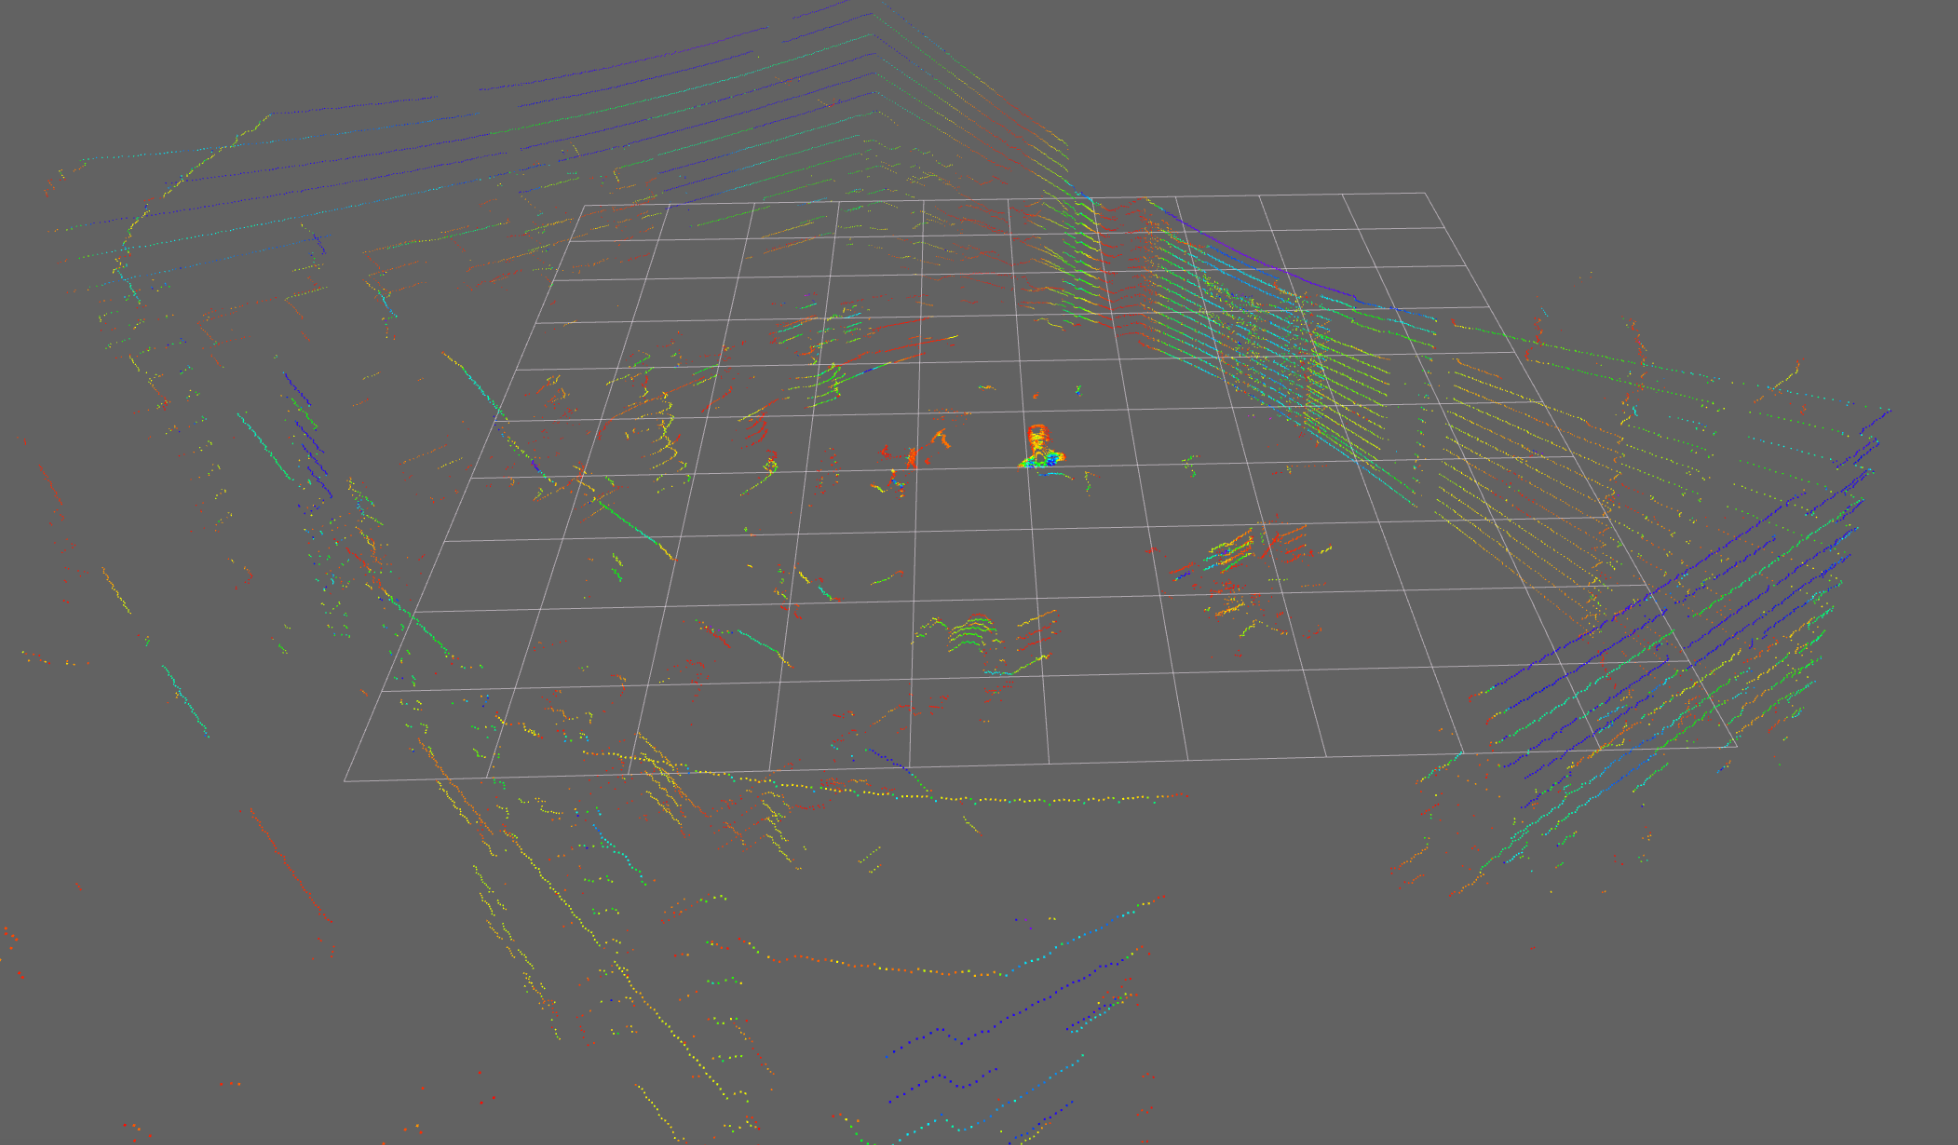
\includegraphics[width=0.5\textwidth]{resources/rviz.PNG}
	\caption[PointCloud2 Datenstream mit Rviz]{PointCloud2 Datenstream mit Rviz}
	\label{fig:rviz}
\end{figure} 

Mittels dem ROS-Tool Rviz lässt sich der Datenstream über velodyne\_packets direkt visualisieren. In Abbildung \ref{fig:rviz} ist ein statischer Datenstream visualisiert. Dies geschieht indem das Tool kontinuierlich die Messages empfängt. \textit{(subscribed)}. 

ROS bietet zudem die Möglichkeit über den \textit{rosbag} Befehl, Messungen aufzunehmen und abzuspeichern. Dies ermöglicht somit nicht nur den aktuellen Sensordatenstream zu visualisieren, sondern auch getätigte Messungen zu archivieren \cite{ROSTutorials}. 

\subsection{Schlussfolgerung}
Für die Aufgabenstellung eignet sich ROS gut, wegen den bereitstehenden Tools und den Packages, mit denen ein grosser Teil der Software abstrahiert werden kann. Der aktuelle Code muss um einige Nodes erweitert werden. Die einzelnen Sensordaten werden einerseits auf die aktuelle Position verschoben und anderseits zu einer einzigen Punktwolke zusammengefüg. Die Einarbeitung mit ROS ist jedoch relativ umfangreich und bietet eine Vielzahl an Tools, die zuerst kennen gelernt werden müssen.  

\section{Datenverarbeitung}
\label{sec:Datenverarbeitung}
Um die Datenmenge zu verarbeiten und die Ansteuerung der Komponenten zu realisieren, eignen sich Einplatinencomputer. Einplatinencomputer besitzen den Vorteil, dass sie gegenüber üblichen Mikroprozessoren grössere Speichermöglichkeiten, höhere Prozessorleistungen und bootbare Betriebssysteme ermöglichen. Gegenüber \ac{XPC} besitzen sie den Vorteil, dass sie Hardware näher sind, indem sie direkt ansteuerbare Pins besitzen (GPIOs). Aus diesem Grund werden nachfolgend diverse Einplatinencomputer betrachtet. Kriterien bei der Auswahl eines geeigneten Boards sind Prozessorleistung, \ac{RAM}, Preis, Ethernet-Schnittstelle, Speichermöglichkeit, GPIO-Verfügbarkeit und die verbaubare Dimension. Diese Kriterien wurden durch die Vorgaben des Pflichtenhefts im Anhang \ref{Pflichtenheft} festgelegt. Geeignete Prozessorleistung, Speichermöglichkeit und \ac{RAM} sind für die erfolgreiche Verarbeitung der Sensordaten nötig, da die Punktwolke mit zunehmender Zeit an Datengröße zunimmt. Die Datenübermittlung des Velodyne und des Packpots erfolgt über Ethernet, daher benötigt der Einplatinencomputer mindestens einen RJ45-Anschluss.

\subsection{Raspberry Pi 2 \& 3}
\label{subsec:Raspberry}
Das Raspberry Pi ist eines der bekanntesten Einplatinencomputer und bietet daher eine grosse Community. Da bereits ein Raspberry Pi 2 zur Verfügung gestanden ist, konnten die ersten Erfahrungen mit einem Raspberry Pi gemacht werden. Das Raspberry bietet zusammen mit ROS Kinetic Kame und Ubuntu Mate LTS 16.04 eine Lösung für die Datenverarbeitung. Das Raspberry Pi 2 bzw. 3 basiert auf einem Broadcom \ac{SOC} und ist mit einem \ac{ARM} Cortex A7 bzw. A53 Prozessor mit vier Kernen ausgestattet. Die Taktfrequenz liegt bei diesem lediglich bei 1.2 GHz. Beide Modelle besitzen 1 GB \ac{RAM}. Das Betriebssystem wird auf einer \ac{SD} gebootet. Speichermöglichkeiten sind über USB oder die SD-Karte vorhanden. Auch GPIOs und eine Ethernetschnittstelle sind beim Raspberry Pi vorhanden. Der Preis eines Raspberry Pi liegt momentan bei ca 50 Fr. \cite{rpi}

\subsection{Banana Pi M3}
\label{subsec:BananaPi}
Der Banana Pi M3 bietet zur Zeit (Stand Oktober 2017) die höchste Performance bei Einplatinencomputern mit \ac{ARM}-Architektur durch den Allwinner A83T Achtkern-Prozessor, der mit 1.8 GHz taktet und den 2 GB RAM. Neben USB-Anschlüssen bietet es eine SATA-USB-Schnittstelle, die den internen 8 GB \ac{eMMC}-Speicher um bis zu 2 TB erweitern lässt. Es bietet auch direkt integrierte WLAN-Schnittstellen, sowie eine RJ45 Gigabit Netzwerkschnittstelle. Der Preis eines BananaPi M3 liegt momentan bei ca 90 Fr.. Im Zusammenhang mit Banana Pi M3 und Ubuntu werden mehrfach Komplikationen und Probleme veröffentlicht \cite{rpi} \cite{banana}. Dies ist ein bedeutender Nachteil für dieses Einplatinencomputer. 

\subsection{Odroid C2 \& XU4} 
\label{subsec:Odroid}
In diversen Literaturen (siehe \cite{ROSprojects} Kapitel 4) werden neben dem Raspberry Pi, Odroid Boards als empfohlene Einplatinencomputer aufgelistet. Dabei stehen die aktuelle Modelle Odroid-C2 oder Odroid-XU4 zur Verfügung. Sie bieten eine höhere Prozessorleistung, 1.5 GHz bzw. 2 GHz mit je 2 Gigabyte \ac{RAM}. Betriebssysteme können via \ac{SD} oder \ac{eMMC} gebootet werden. Beide Boards sind jedoch noch nicht lange auf dem Markt und bieten in vielen Anwendungen nur Beta-Versionen. Vor allem die Unterstützung von Ubuntu LTS 16.04 ist nicht restlos geklärt. Der Preis dieser Boards ist ca. 80 - 90 Franken \cite{rpi}.

\subsection{Up Board Squared} 
\label{subsec:Up Board Squared}
Dieser Einplatinencomputer unterscheidet sich wesentlich von den bisherig betrachteten Boards. Der Prozessor arbeitet nicht mit \ac{ARM}-Architektur, sondern mit \ac{AMD64}-Architektur. Somit können Ubuntu und ROS Distributionen voll umfänglich genutzt werden. Er besitzt mit Intel Pentium ein vier kerniger Prozessor und taktet mit 2.5 GHz. Zusätzlich bietet er einen separaten 500 MHz \ac{GPU} und bis zu 8 GB \ac{RAM}. Neben USB werden auch zwei RJ45-Schnittstelle und ein GPIO Pinlayout angeboten, welches dem des Raspberry Pis entspricht. Das Up Board Squared bietet sich an, falls die Performance und die Kompatibilität der ARM-Architektur mit ROS nicht ausreicht. Der Preis eines Up Board Squared kostet je nach Ausführung zwischen 180-380 Fr.

\subsection{Schlussfolgerung}
\label{subsec:Schlussfolgerung}
Für die Aufgabenstellung eignet sich lediglich das Raspberry Pi 2 oder 3, um ROS mit Ubuntu LTS 16.04 zu betreiben. Das Banana Pi und die Odroid Boards sind im Kriterium Speichermöglichkeit und Prozessorleistung besser geeignet, können jedoch wegen fehlender Betriebsystem-Kompatibilität nicht genutzt werden. Die Dimensionen aller betrachteten Boards sind, mit Ausnahme des Up Board Squared sehr kompakt. Im Punkt Ethernetschnittstelle bietet lediglich das Up Board Square zwei Ethernetanschlüsse, mit welchen ein zusätzlicher Ethernet Switch hinfällig wird. Das Up Board Squared bieten in fast allen Kriterien eine bessere Lösung. Aus Kostengründen wurde für den zu erarbeitenden Prototypen das Raspberry Pi als genügend bewertet. Für eine allfällige Optimierung bietet sich das Up Board Squared an.

\section{Antriebsmöglichkeiten}
\label{sec:Antriebsmoeglichkeiten}
Um den Velodyne VLP-16 um eine Achse drehen zu lassen, müssen Motoren eingesetzt werden. Nachfolgend werden zwei verschiedene Motorenarten beschrieben, die sich für die Aufgabenstellung eignen. Wichtige Kriterien für die Aufgabenstellung sind einerseits die Ansteuerung und die Dimension. Anderseits muss die Möglichkeit bestehen die Winkeländerung zu eruieren. 

\subsection{Schrittmotor}
\label{subsec:Schrittmotor}
Der Schrittmotor ist eine Antriebsmöglichkeit, welche für das Projekt in Frage kommt. Es gibt sehr kostengünstige und kompakt dimensionierte Motoren dieser Art. Ein interessanter Aspekt ist das gezielte Steuern des Motors. Durch einen Stromimpuls bewegt sich ein Schrittmotor nur einen festgelegten Winkelschritt weiter. Er kann bereits ohne zusätzliche Sensorik definierte Schritte anfahren, aus denen die Winkeländerung eruiert werden kann. Schrittmotoren besitzen die Eigenschaft, dass in der Ruhelage ein Haltemoment entsteht. Diese Eigenschaft wird jedoch für die Aufgabenstellung nicht zwingend benötigt. Preislich muss bei einem geeigneten Schrittmotor mit 40 Fr. gerechnet werden. 

Nachteilig für die Aufgabenstellung am Schrittmotor ist der höhere Stromverbrauch, vor allem zum Aufbringen des Haltemoments. Da nur ein Schritt ausgeführt wird, wenn das entsprechende Drehmoment nicht überschritten wird, müsste dieses sorgfältig berechnet werden. Ein bedeutender Nachteil im Zusammenhang mit der Aufgabenstellung ist, dass durch Schrittverluste die Winkeländerung nicht mehr quantitativ ermittelt werden kann. Schrittmotoren mit integrierten Encodern würden in diesem Fall Abhilfe schaffen. Aus Kostengründen (Preise ab 300 Fr. \cite{mouserstepper}) wurden Schrittmotoren mit integrierten Absolutencodern nicht weiter vertieft. 
Ein weiterer Nachteil ist das verhältnismäßig hohe Gewicht. Dies ist kein Kriterium für die Aufgabenstellung, sollte jedoch bei der Realisierung beachtet werden.

Um mit einem Einplatinencomputer einen Schrittmotor anzusteuern, empfiehlt sich ein Schrittmotorentreiber. Mit solchen Treibern lässt sich der Motor mittels 2 Steuerpins rotieren. Um die Drehgeschwindigkeit zu senken, bieten diese Treiber die Möglichkeit, die Schritte in 2, 4, 8 und 16 Teilschritte zu senken. Es ermöglicht zudem eine feinere Bewegung. \cite{DRV8825}.

\subsection{Gleichstrommotor}
\label{subsec:Gleichstrommotor}
Als Alternative zum Schrittmotor bietet sich ein üblicher Gleichstrommotor. Diese Motoren sind für viele Einsatzbereiche geeignet und es gibt sie in verschiedenen Grössen und Umdrehungszahlen. Im Gegensatz zu Schrittmotoren laufen Gleichstrommotoren kontinuierlich, aufgrund eines Stroms, der durch die Wicklungen fliesst. Nachteilig ist somit, dass weder die genaue Anzahl Umdrehungen noch die momentane Phasenlage bekannt ist. Es gibt jedoch eine Vielzahl an Möglichkeiten diese zu eruieren. Einerseits gibt es die Möglichkeit mittels Hall-Sensoren oder mittels Quadraturencodern, die aktuelle Drehrichtung und die Drehzahl zu ermitteln. Um dies zu ermöglichen, braucht es zusätzlich einen Vierquadrantensteller (H-Brücke), sowie eine Sensorlogik, damit der Sensor mittels \ac{PWM} angesteuert werden kann. Im Preissegment um 40 Fr. gibt es leistungsfähige Gleichstrommotoren für den Anwendungsbereich \cite{pololumotor}.

\section{Positionsbestimmung}
\label{sec:position}
Damit die Messdaten des Velodyne auf eine feste Koordinatenachse abgebildet werden können, benötigt eine drehende Konstruktion eine absolute Positionsbestimmung. Nachfolgend sind Varianten erläutert, welche sich dafür eignen.

\subsection{LED und Photodiode}
\label{sec:LED}
Eine simple Variante ist der Einsatz einer LED, welche im rotierenden Teil konstant leuchtet. Dabei wird die Photodiode an den stationären Teil angebracht und als Nullpunkt genutzt. Durch das Licht der LED wird ein Strom an die Photodiode übertragen und dies kann mit einer einfachen Beschaltung über einen GPIO gemessen werden. Nachteilig bei dieser Variante ist der Lichtkegel der LED. Die LED müsste so verbaut werden, dass ein fokussierter Lichtstrahl auf die Photodiode fällt. Ansonsten kann der  Nullpunkt stark abweichen. Zudem ist diese Variante sehr stark abhängig vom Umgebungslicht. Diese Variante bedingt, dass mittels einer weiteren Komponente die Winkeländerung gemessen werden kann.

\subsection{Sensor QRE 1113}
\label{sec:QRE}
Eine weiter ähnliche Variante ist der Einsatz eines QRE 1113 Sensors. Dieser Sensor baut auf dem Prinzip der Infrarotreflektion auf. Dabei werden dunkle Oberflächen schlechter reflektiert, als helle Oberflächen. Diese Eigenschaft wird genutzt, um den Nullpunkt zu detektieren. Auch diese Variante bedingt, dass mittels eines weiteren Komponenten die Winkeländerung gemessen werden kann.

Eine weitere Variante ist die Aneinanderreihung dieser Sensoren. Dies bietet die Möglichkeit einen absoluten Encoders mit Binär- oder Gray-Code, wie in Abbildung \ref{fig:Encoder} dargestellt, zu realisieren. Es können mit N Sensoren 2$^N$ Zustände unterschieden werden. Aus den Zuständen kann der Winkel berechnet werden. Für diese Aufgabe werden jedoch N GPIOs benötigt.
\begin{figure}[H]
	\centering
	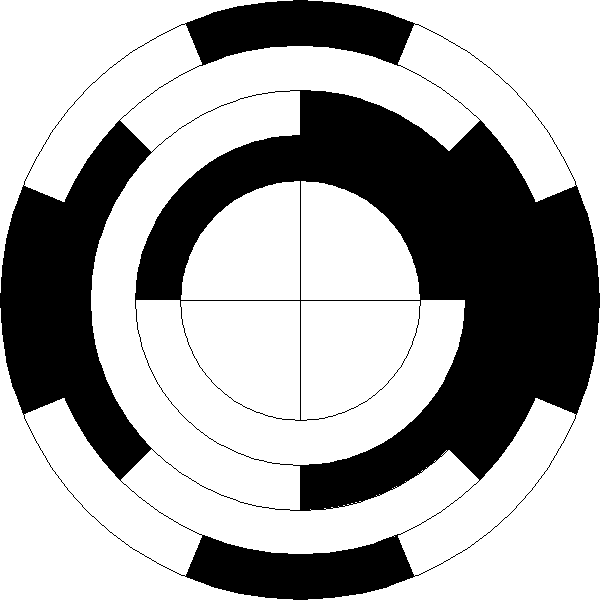
\includegraphics[width=0.25\textwidth]{resources/encoder.png}
	\caption[Quadraturencoder mit 4 Sensoren]{Quadraturencoder mit 4 Sensoren}
	\label{fig:Encoder}
\end{figure} 

Auch diese Variante ist stark abhängig vom Umgebungslicht und zusätzlich können die einzelnen Sensoren einander durch Streuung beeinflussen. Um dies zu minimieren, sollte der Absolutencoder mittels Gray-Code realisiert werden, damit nur immer eine gleichzeitige Zustandsänderung stattfindet. Die Abtastung der Zustände muss nach dem Nyquist-Shannon-Abtasttheorem mit mindestens doppelter Abtastfrequenz gemessen werden.
 
\section{Speisung und Verkabelung}
\label{sec:Speisung und Verkabelung}
Dieses Kapitel erläutert weitere Komponenten, welche je nach Konzept nötig sind, um  die Speisung und Verkabelung zu ermöglichen.

\subsection{Abwärtswandler}
\label{subsec:Abwaertswandler}
Der Abwärtswandler D24V50F5 von Pololu eignet sich sehr gut für die Stromversorgung von Einplatinencomputern. Er bietet eine stabile 5 Volt Ausgangsspannung bis zu einer ausgangsseitigen Belastung von 8 Ampere. Der Wirkungsgrad beläuft sich dabei auf über 90 Prozent bei einer eingesetzten Betriebsspannung von 12 Volt. Diese Angaben gehen aus Abbildung \ref{fig:D24V50F5} hervor, die aus dem Datenblatt des Abwärtswandlers stammen.\cite{D24V50F5}
\begin{figure}[H]
	\centering
	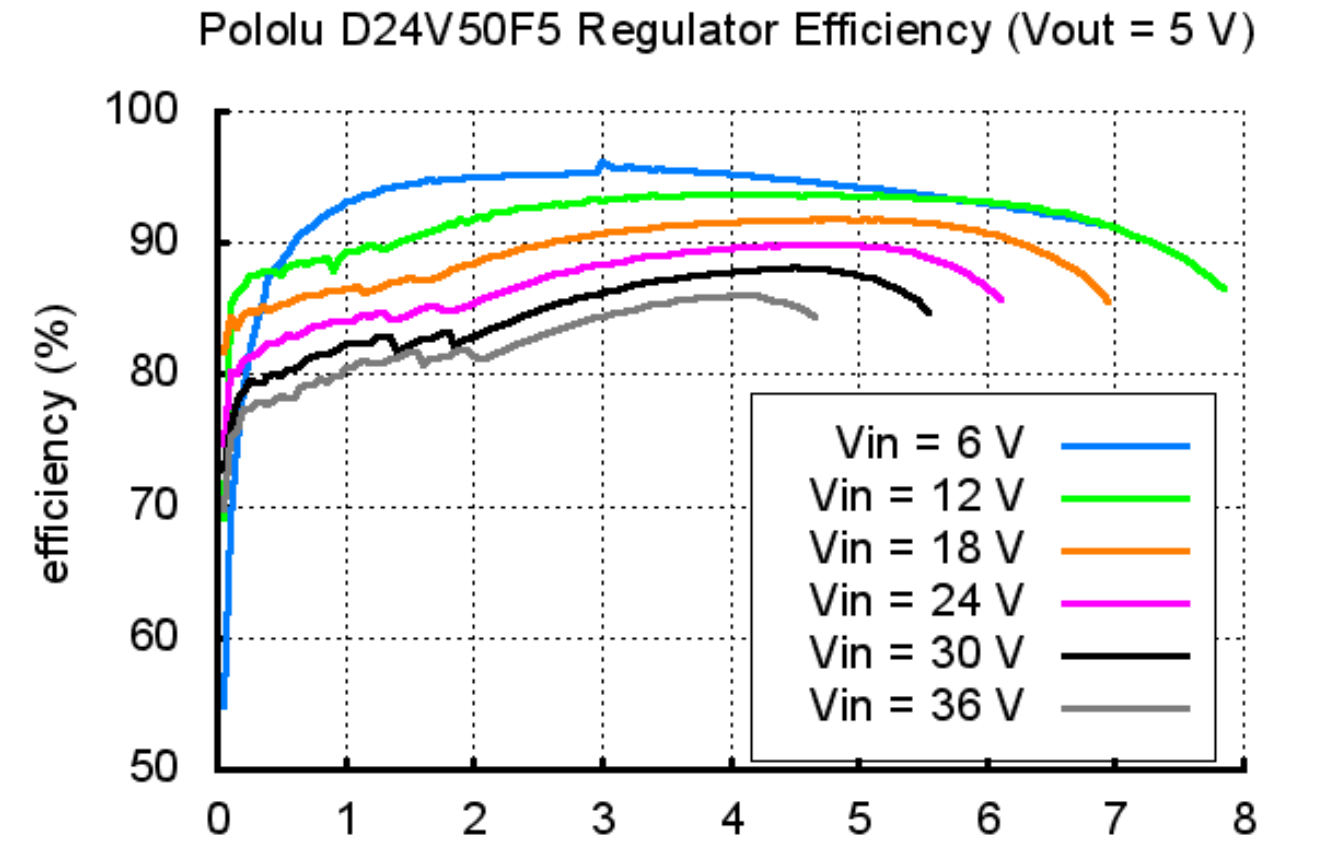
\includegraphics[width=0.4\textwidth]
	{resources/D24V50F5.PNG}
	\caption[Wirkungsgrad D24V50F5]{Wirkungsgrad D24V50F5 \protect\cite{D24V50F5}}
	\label{fig:D24V50F5}
\end{figure}

\subsection{Ethernet Schleifring}
\label{subsec:Schleifring}
Da übliche Kabel nur für einige wenige Verdrehungen ausgelegt sind und so bei drehenden Vorrichtungen kaputt gehen, wird ein Schleifring als Drehübertrager eingesetzt. Ein Schleifring überträgt das Eingangssignal über eine Bürste und bildet somit einen Gleitkontakt. Die Problematik liegt beim Velodyne VLP-16, dass die Datenübertragung über Ethernet übermittelt werden muss. Gängige Schleifringe bieten kein Gewähr für die Übertragung von Ethernet, da die Datenrate verhältnismässig hoch ist. Es gibt jedocu einige wenige Hersteller aus dem amerikanischen und asiatischen Markt, welche Ethernet-Übertrager vertreiben. Ein Ethernet-Schleifring, der zusätzlich Leistungsübertragung bis 5 Ampere zulässt kostet nach Abklärungen bei diversen Herstellern zwischen 120 - 600 Fr.  

\subsection{Ethernet Switch}
\label{subsec:Ethernetswitch}
Die Einplatinencomputer aus Kapitel \ref{sec:Datenverarbeitung} benötigen mit Ausnahme des Up Board Squared ein weiteren Ethernetanschluss, damit die Kommunikation gewährleistet ist. Ethernet Switches gibt es in diversen Variationen und Grössen. Für die Aufgabenstellung wird ein möglichst kompakter Switch benötigt, der mindestens drei Anschlüsse bietet. Im Preissegment von 30Fr. können bei Mouser, Distrelec und Farnell sehr kompakte 5-Port Switch bestellt werden. Eine gute Lösung ist dafür der Ethernet Switch GS105 der Marke Netgear. Dieser benötigt einen 12 Volt Speisung, mit dem sich eine Spannungsanpassung erübrigen würde. Zudem ist er im direkten Vergleich das Produkt mit den kleinsten Abmessungen.

\section{Zwischenfazit}
\label{ZwischenfazitInfo}
Für die Einarbeitung in das Projekt ist die Informationsbeschaffung bzw. Recherche ein wesentlicher Bestandteil. Dabei werden wichtige Grundlagen für die Konzeption geschaffen. ROS bietet für 3D Mapping gute Tools und vereinfacht die Datenverarbeitung des Velodyne VLP-16 bedeutend. Mittels Schrittmotoren oder Gleichstrommotoren kann der Velodyne gedreht werden. Mit entsprrechender Sensorik können damit die räumliche Messungen erfolgen. Für die Datenverarbeitung stehen mehrere Einplatinencomputer zur Verfügung, dabei müssen diese jedoch die Kriterien erfüllen. Für endlos drehende Vorrichtungen wird zusätzlich ein Ethernet Schleifring benötigt, da ansonsten die Kabelführung nicht gewährleistet ist.  

